\documentclass[11pt,a4paper]{article}
\usepackage[margin=22mm]{geometry}
\usepackage{graphicx,booktabs,amsmath,hyperref}
\renewcommand{\thefigure}{S\arabic{figure}}
\renewcommand{\thetable}{S\arabic{table}}
\title{Supplementary material: Complete-sizing sensitivity to stress-filter radius}
\author{Supplementary material}
\date{19 November 2026}
\begin{document}
\maketitle
The 16-rib reference layout uses spars at 10\% and 70\% chord and 42,216 shell elements. Each case starts at uniform 10~mm total thickness. Only the filter radius changes; all other analysis and sizing settings remain fixed. The 0.30~m case reuses the audited saved baseline. The new cases were solved to the same own-radius stress and linear-buckling criteria.

Table~\ref{tab:cross} evaluates every final raw stress field at all three radii. Rows identify independently sized designs; columns identify postprocessing measures. These values are scalar averages and do not establish local-strength safety.
\begin{table}[h]\centering
\caption{Final stress fields evaluated at common radii: maximum filtered stress (MPa).}\label{tab:cross}
\begin{tabular}{rrrr}\toprule
Sizing radius (m) & Evaluation 0.15~m & Evaluation 0.30~m & Evaluation 0.60~m\\\midrule
0.15 & 298.869 & 291.615 & 289.813\\
0.30 & 353.220 & 298.027 & 290.456\\
0.60 & 420.128 & 346.857 & 299.169\\
\bottomrule\end{tabular}\end{table}
Table~\ref{tab:effort} reports solved-state counts and measured times. Buckling counts include the initial check of each final FSD design. All FSD stages stop by feasible mass stagnation. Each case uses one uniform-core restoration step; 0.15~m reaches the energy-correction limit, whereas 0.30 and 0.60~m trigger restoration through near-feasible stagnation. Baseline timings are retained from its original run.
\begin{table}[h]\centering\small
\caption{Complete-sizing effort.}\label{tab:effort}
\begin{tabular}{rrrrr}\toprule
Radius (m) & FSD states & Buckling states & Solver time (min) & Wall time (min)\\\midrule
0.15 & 60 & 42 & 150.67 & 153.28\\
0.30 & 24 & 33 & 78.04 & 79.61\\
0.60 & 16 & 35 & 79.81 & 81.11\\
\bottomrule\end{tabular}\end{table}
\noindent Reinforced area sums shell reference areas where either individual face or core thickness grows by more than $10^{-9}$~m from the case's final FSD design. Global growth steps yield 98.45~m$^2$ (100\%) in every case. This includes all shell surfaces, not projected wing area. Figure~S8 describes the distribution of added thickness using descriptive thresholds, not acceptance thresholds.
\setcounter{figure}{2}

\clearpage
Figure~S3 shows the solved-state histories for each radius. Buckling is evaluated after FSD; the horizontal axis includes both stages.
\begin{figure}[h]\centering
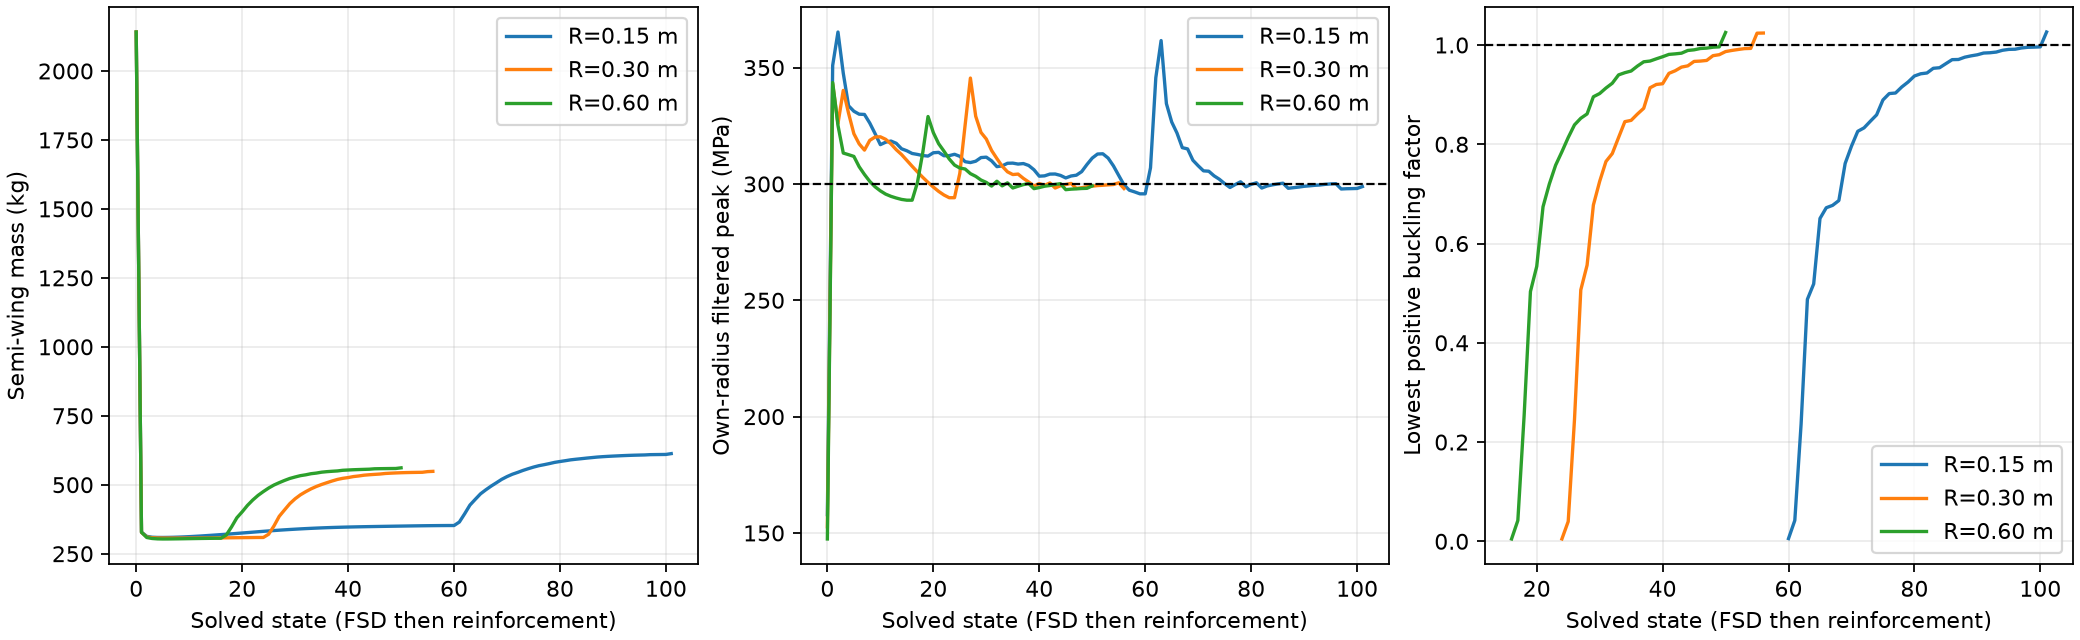
\includegraphics[width=\textwidth,height=0.78\textheight,keepaspectratio]{sizing_histories.png}
\caption{Sizing histories. Filtered peaks use the sizing radius of each design; dashed lines indicate the 300~MPa stress limit and unit buckling factor.}
\end{figure}

\clearpage
Figure~S4 compares the final total-thickness distributions on both skins.
\begin{figure}[h]\centering
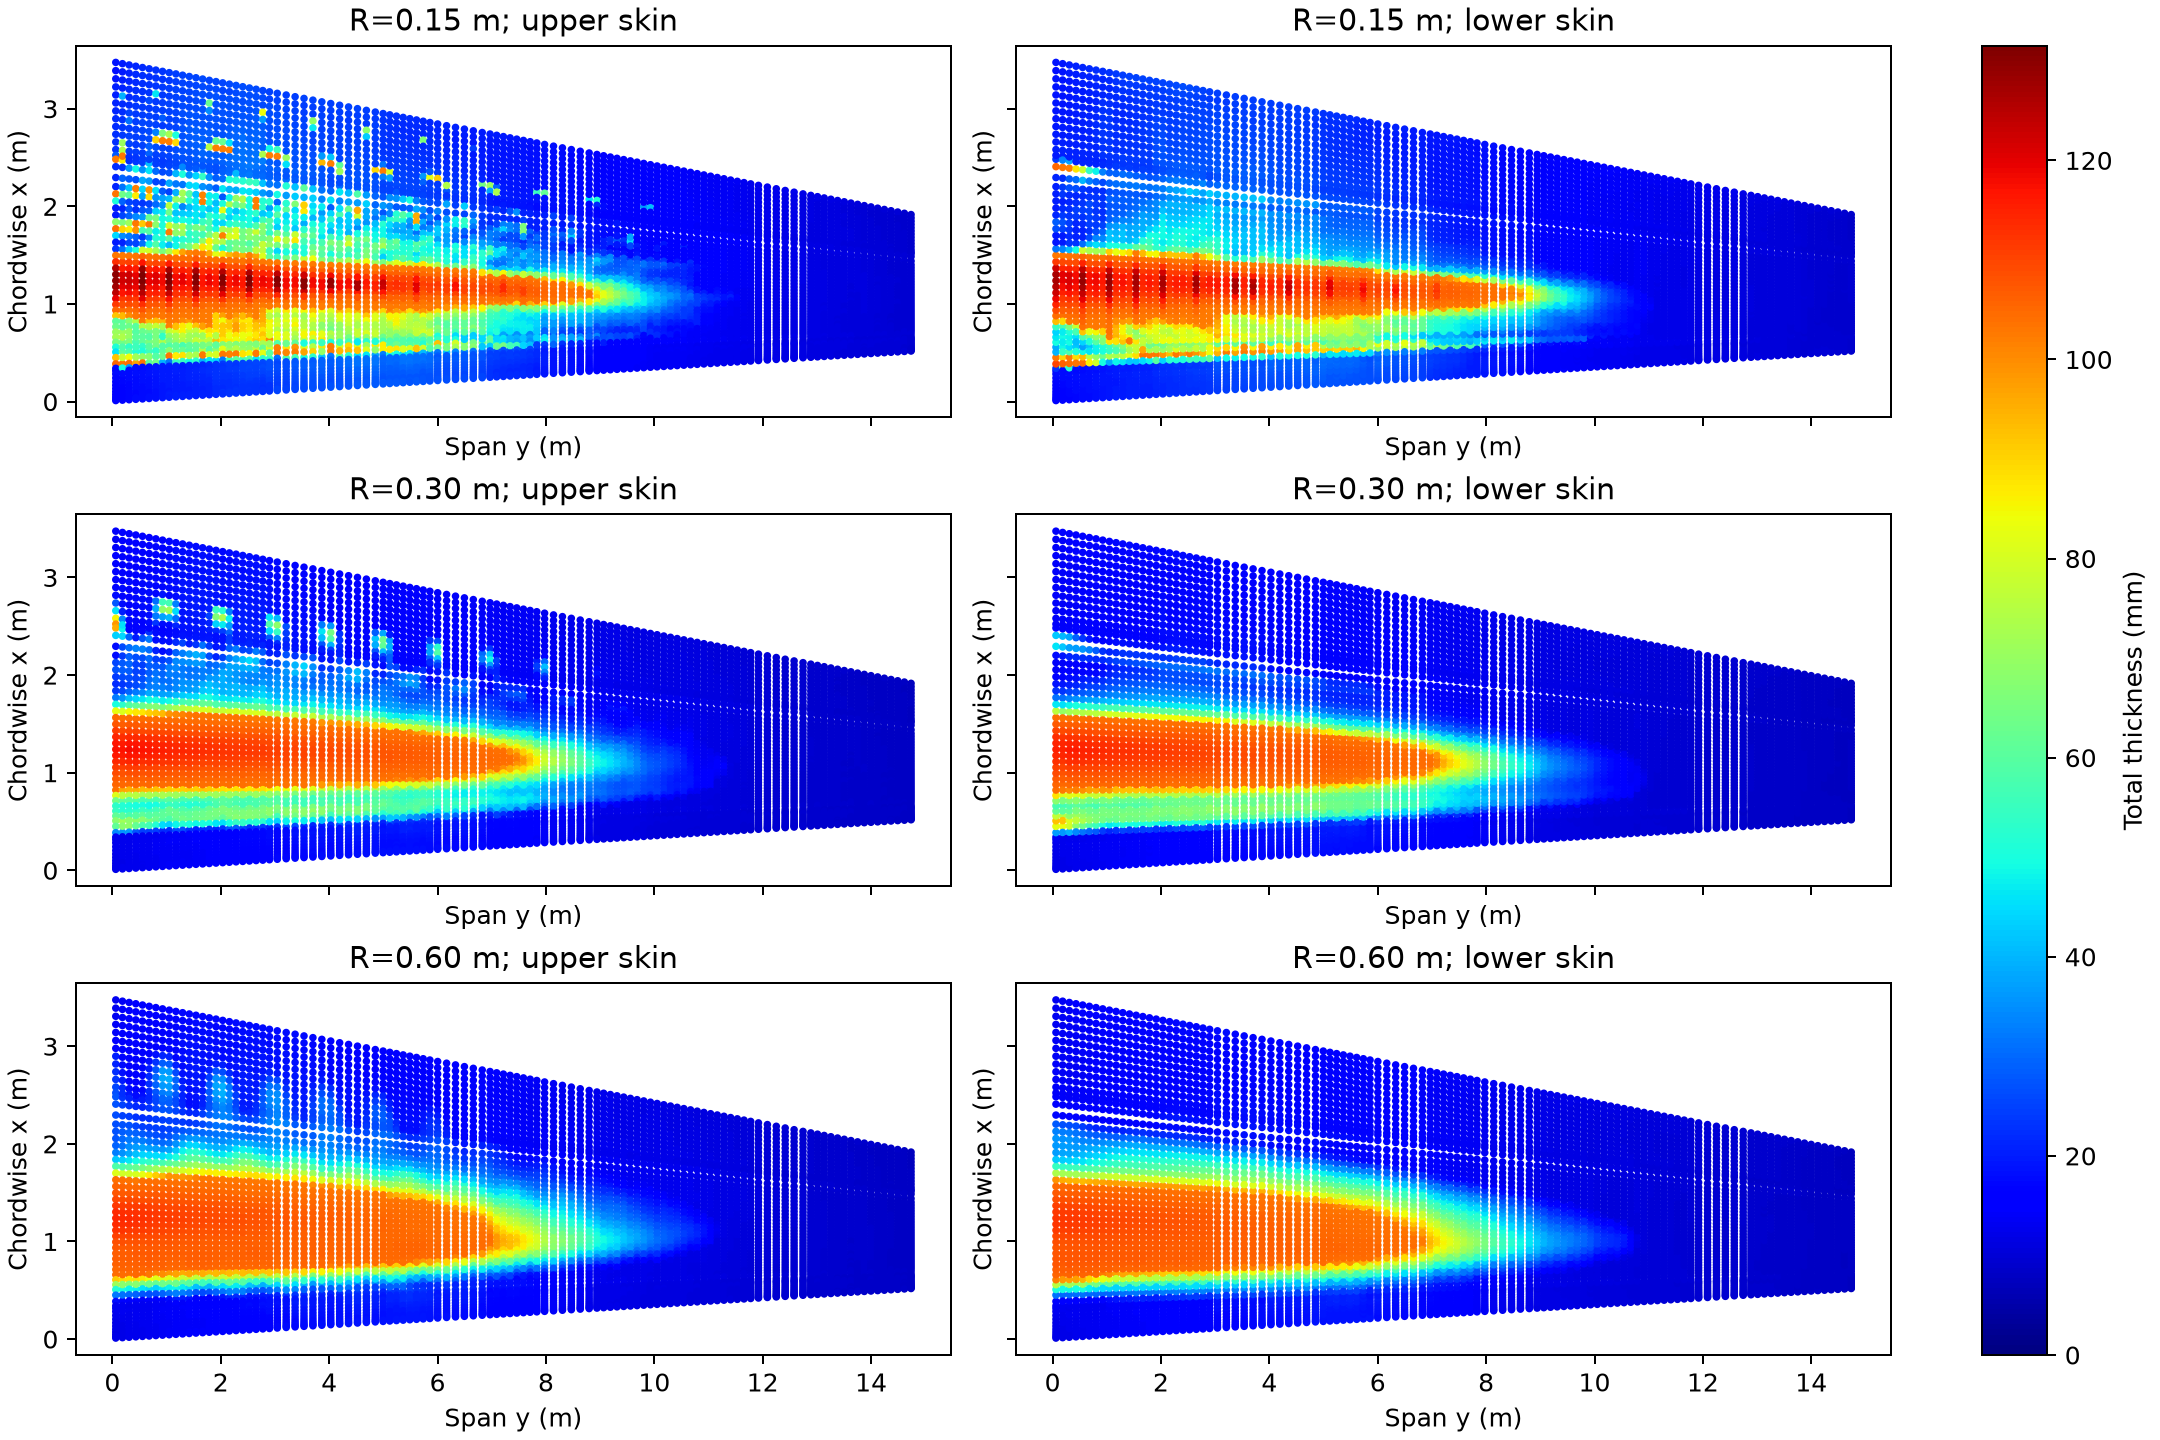
\includegraphics[width=\textwidth,height=0.78\textheight,keepaspectratio]{total_skin_maps.png}
\caption{Final total sandwich thickness on both skins at the three sizing radii, using a shared linear scale. These diagnostic maps show element-centre values.}
\end{figure}

\clearpage
Figure~S5 isolates the thickness of each equal metal face.
\begin{figure}[h]\centering
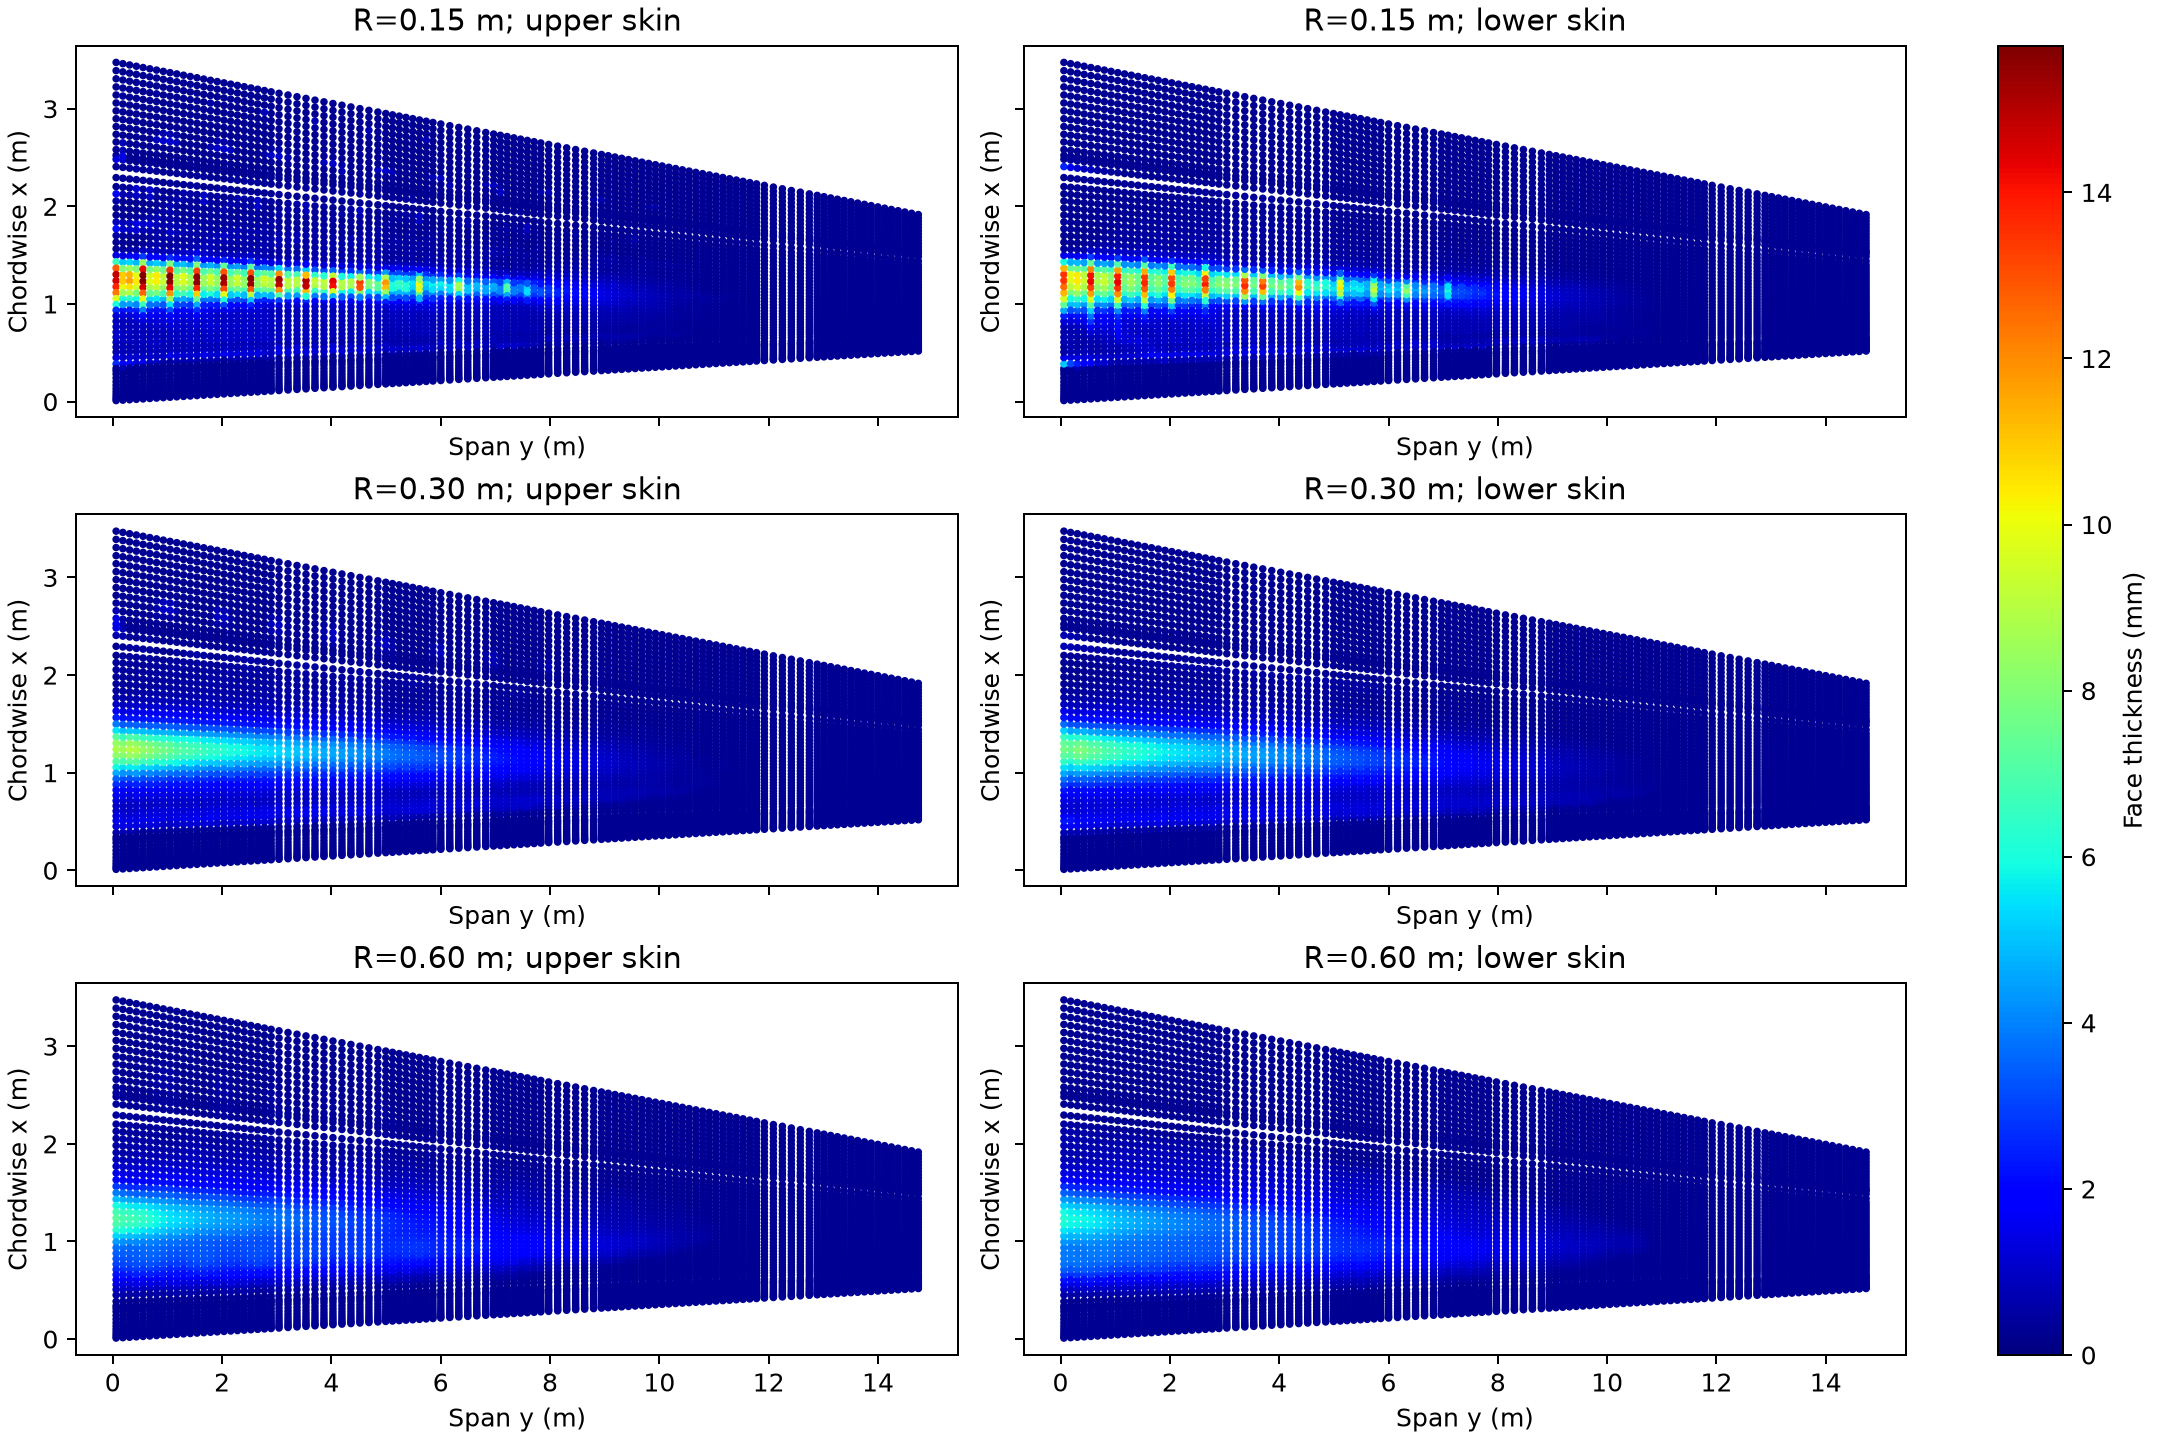
\includegraphics[width=\textwidth,height=0.78\textheight,keepaspectratio]{face_skin_maps.png}
\caption{Final individual-face thickness on both skins, with one shared linear scale.}
\end{figure}

\clearpage
Figure~S6 compares the core-thickness distributions.
\begin{figure}[h]\centering
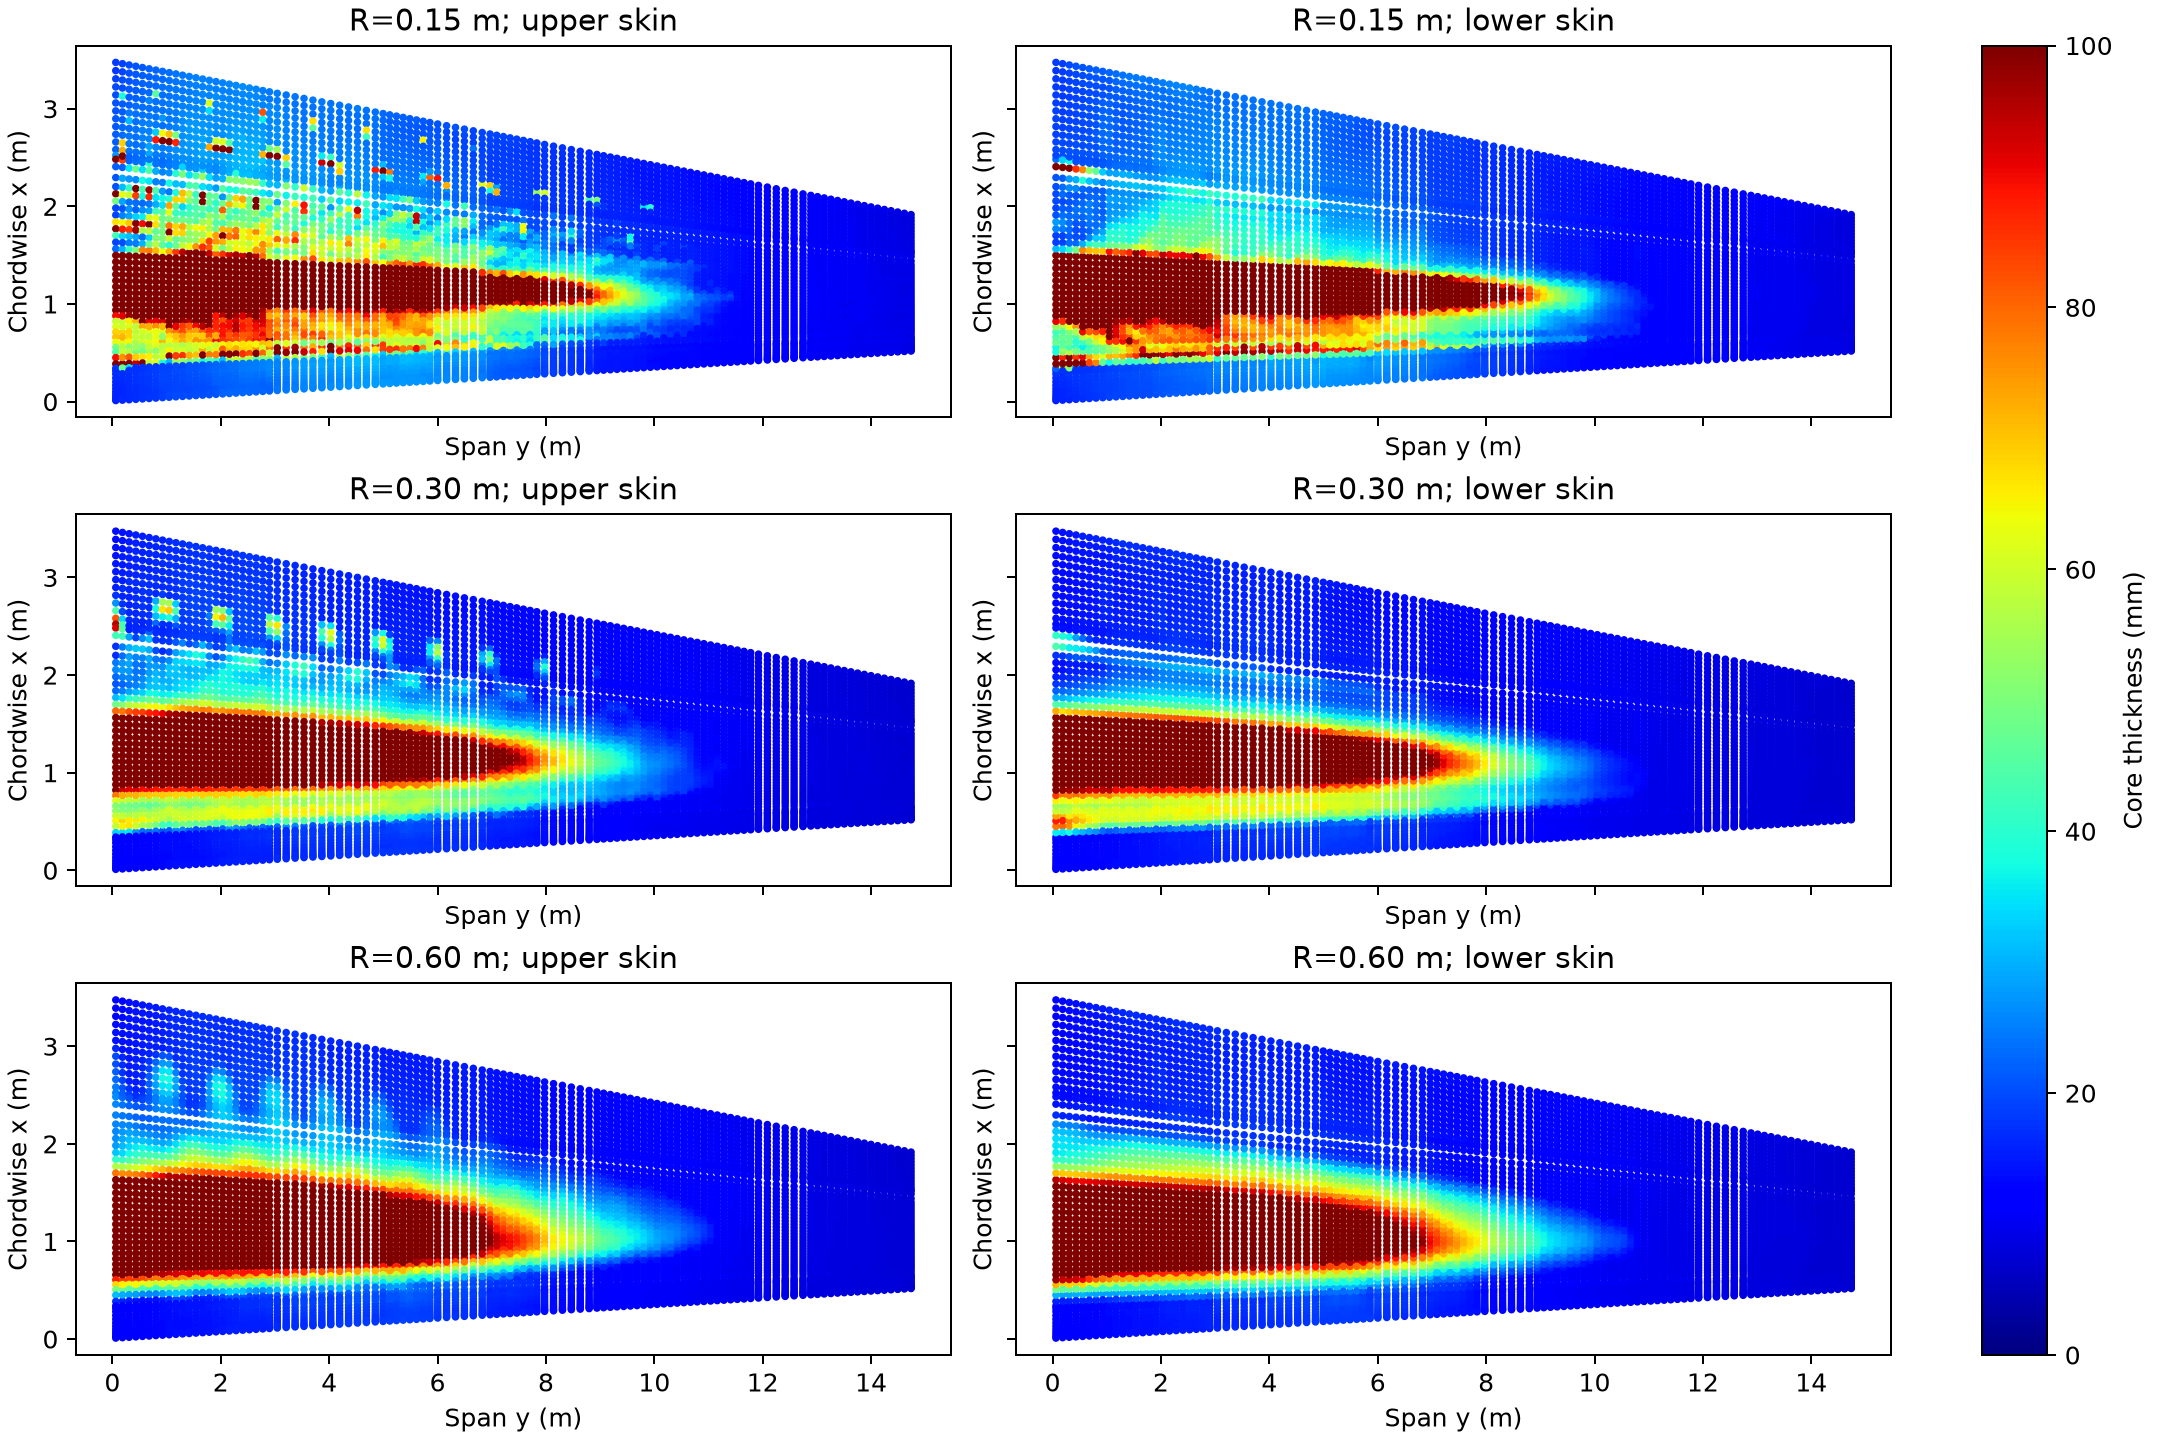
\includegraphics[width=\textwidth,height=0.78\textheight,keepaspectratio]{core_skin_maps.png}
\caption{Final core thickness on both skins; every radius case reaches the 100~mm core bound.}
\end{figure}

\clearpage
Figure~S7 shows the total thickness added during buckling reinforcement relative to each case's own final FSD design.
\begin{figure}[h]\centering
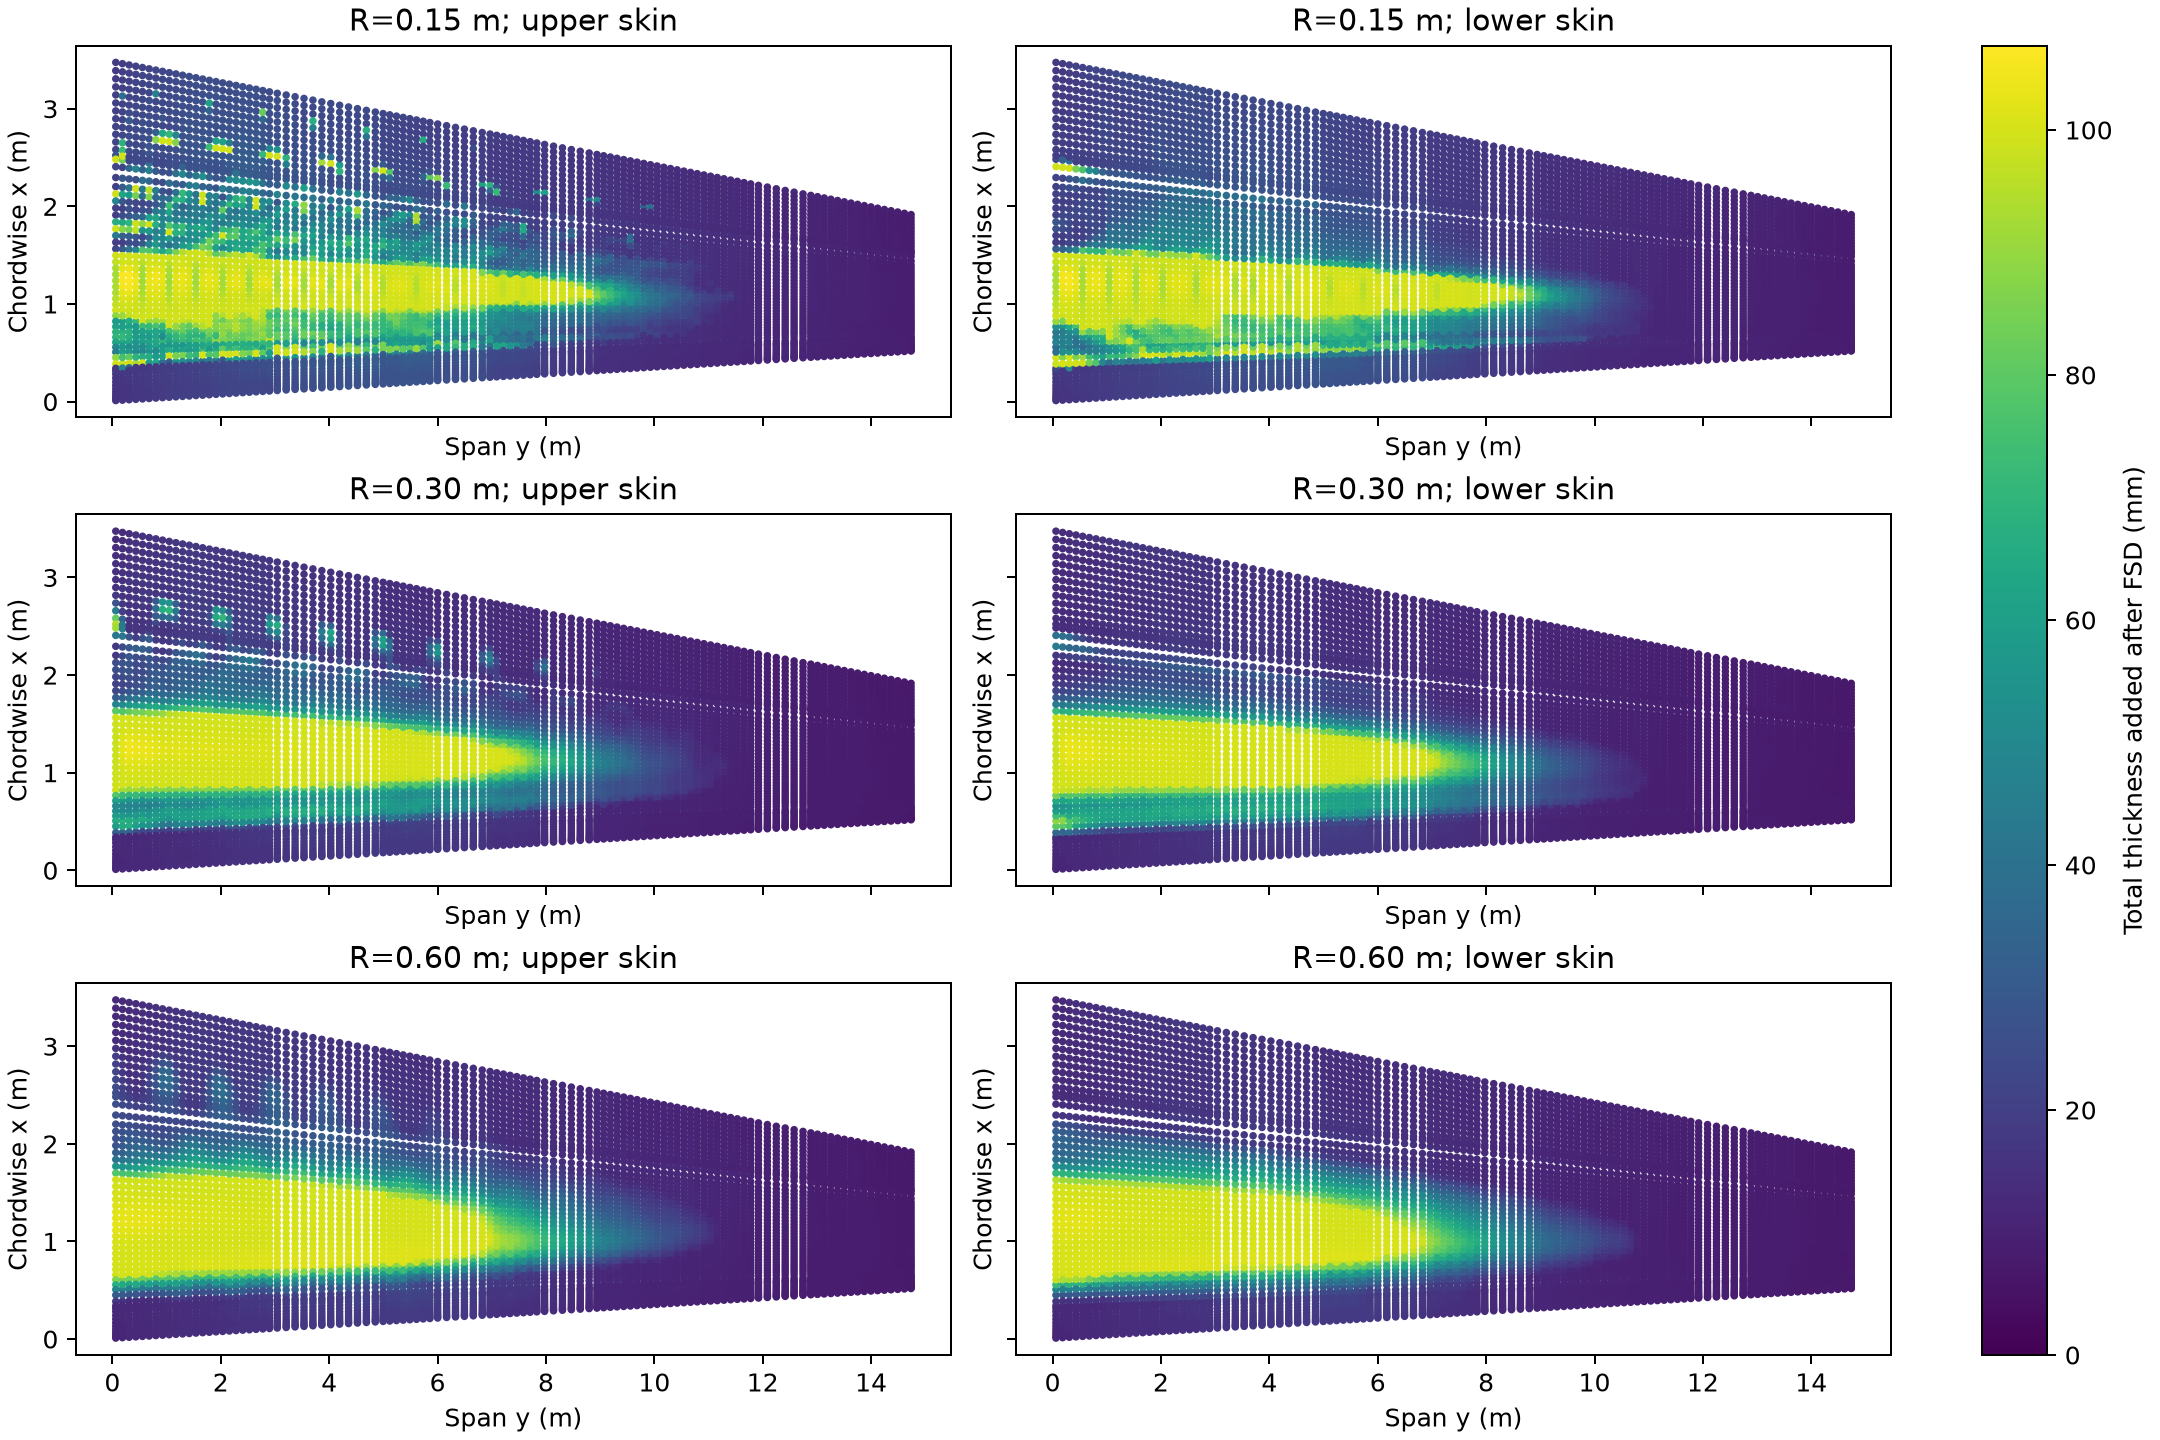
\includegraphics[width=\textwidth,height=0.78\textheight,keepaspectratio]{reinforcement_skin_maps.png}
\caption{Thickness added after FSD on both skins. A common scale distinguishes the amount and spatial distribution of reinforcement.}
\end{figure}

\clearpage
Figure~S8 reports the fraction of all shell reference area exceeding each added-thickness threshold.
\begin{figure}[h]\centering
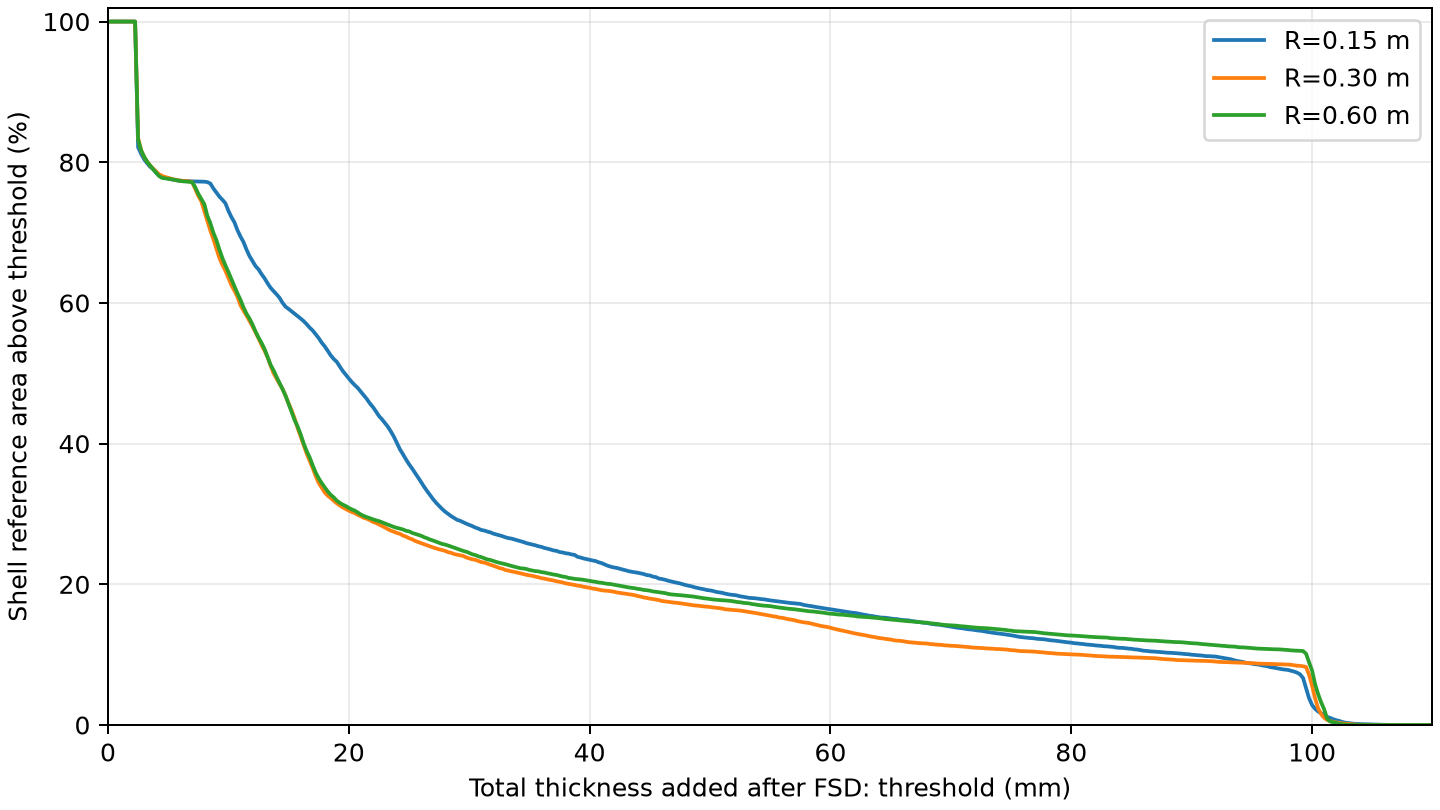
\includegraphics[width=\textwidth,height=0.78\textheight,keepaspectratio]{reinforcement_area_distribution.png}
\caption{Area distribution of total thickness added after FSD. Thresholds describe the saved fields; they are not feasibility criteria. The curves quantify spatial differences despite the common 100\% any-growth area.}
\end{figure}
\end{document}